% !TeX root = ../../main.tex
\section{Model implementation}
\label{sec: modelimplementation}
COMSOL was selected for detailed reactor modelling, utilising the CFD and Heat Transfer modules \cite{comsol_comsol_2020,comsol_cfd_2020,comsol_heat_2020}. A single tube of the reactor was modelled in 2D axisymmetric geometry.

\subsection{Physics setup}
The physics interfaces used to model each zone of the reactor, as well as assumptions made in modelling, are outlined below. Further details of the equations implemented are available in \cref{app:comsol}.

\subsubsection{Reaction zone}

Within this zone, nonisothermal flow and reacting flow couplings are used to link heat and mass transfer, and chemical reaction with mass transfer, respectively.

\paragraph{Mass transfer: Brinkman equations}
The Brinkman equations describe laminar flow through porous media, and are an extension of Darcy's law \cite{comsol_cfd_2020}. A key parameter is the bed porosity; this was found to be \num{0.277} from the porosity of the sintered SiC support (0.30) and the required catalyst loading of \SI{300}{\kg\per\cubic\m}. Fluid properties (density, viscosity) were taken from Aspen Properties (see \cref{sec:flowsheeting}) and assumed invariant with temperature. Solid permeability was assumed constant at \SI{1e-12}{\square\m}. The inlet boundary condition was set to a uniform velocity profile dividing the required throughput across the 7 reactor tubes. The outlet boundary condition was set to a pressure of \SI{1}{\atm}, as required for donwstream processing.

\paragraph{Chemical reaction: Transport of concentrated species}
Reaction rate laws outlined in \cref{sec:R1-kinetics} were implemented to define the species-wise material balances. Molar concentrations in the inflow stream were defined as determined in Aspen Plus, excluding species of very small concentration.

\paragraph{Heat transfer: Porous media}
A critical parameter for heat transfer in the bed is the overall thermal conductivity. This was found through a volume-average model considering the conductivities of the fluid (\SI{0.187}{\W\per\m\per\K}), catalyst (\SI{3}{\W\per\m\per\K}) and sintered SiC support (\SI{40}{\W\per\m\per\K} at \SI{30}{\percent} porosity \cite{jang_thermophysical_2007}, as opposed to \SI{120}{\W\per\m\per\K} for bulk SiC \cite{accuratus_silicon_2013}) phases within the bed. Upstream reactant temperature was set to \SI{330}{\K}, following Aspen. A convective heat transfer coefficient of \SI{500}{\W\per\square\m\per\K} was defined for the outer boundary of the reaction zone, to model heat removal by the shell-side cooling fluid. Additionally, conduction into the wall of the inner cooling tube was modelled.

\subsubsection{Wall}

The secondary cooling tube runs axially along the centre of the tubular reactor.

\paragraph{Heat transfer: Solid}
The wall medium was modelled as AISI 4340 Steel from the built-in COMSOL materials library, with a thermal conductivity of \SI{44.5}{\W\per\m\per\K}. No conduction from the tube wall into the tube sheets at the ends of the reaction was modelled.

\subsubsection{Coolant zone}

A co-current cooling water flow within the secondary cooling tube serves to remove excess heat from the reaction. A nonisothermal flow coupling links heat and mass transfer.

\paragraph{Mass transfer: $k$-$\varepsilon$ Turbulence model}
Due to the high flow rate through the tube and its small diameter, the flow regime is turbulent. Temperature-dependent fluid density and viscosity are determined from the COMSOL material library. The inlet boundary condition is set to a mass flow of \SI{0.3}{\kg\per\s} and the outlet to a pressure of \SI{1}{\atm}.

\paragraph{Heat transfer: fluid}
Temperature-dependent thermal conductivity of the fluid is found from the COMSOL material library. The inflow boundary condition is set to the mixed coolant stream temperature of \SI{325}{\K} (see \cref{sec:R101-CW}).

\subsection{Optimisation and sensitivity analysis}

\subsubsection{Secondary cooling system sizing}

\begin{figure}[h]
    \centering

    \begin{subfigure}{0.49\linewidth}
        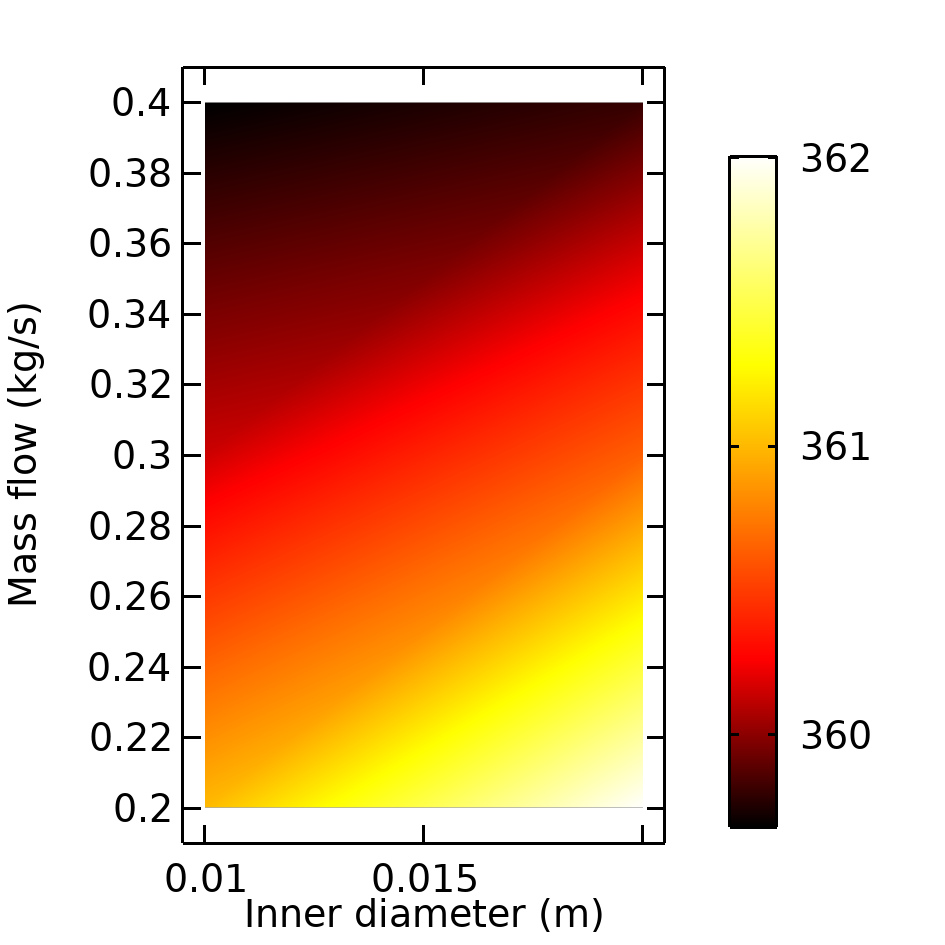
\includegraphics[width=\linewidth]{figures/S2-maxT.png}
        \caption{Maximum temperature reached in the reactor}
        \label{fig:comsol-S2:maxT}
    \end{subfigure}
    \begin{subfigure}{0.49\linewidth}
        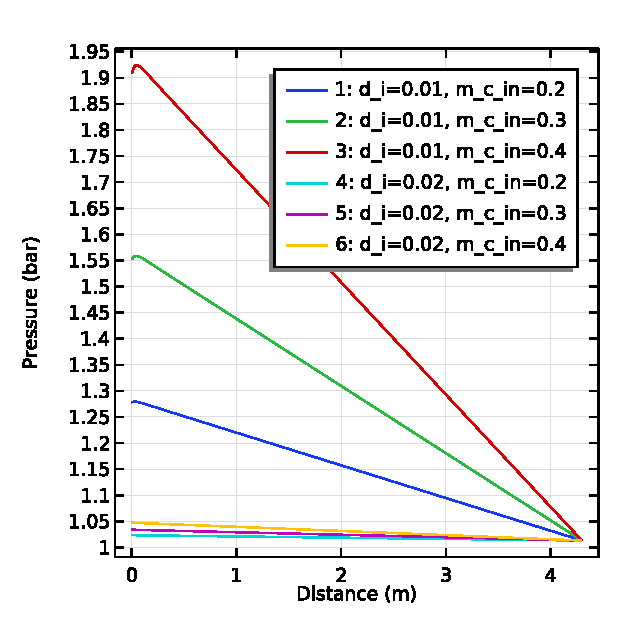
\includegraphics[width=\linewidth]{figures/S2-CW-Pdrop.eps}
        \caption{CW side pressure drop}
        \label{fig:comsol-S2:CW-Pdrop}
    \end{subfigure}

    \caption{Sensitivity to secondary CW parameters}
    \label{fig:comsol-S2}
\end{figure}
Inner coolant flowrate and diameter of inner cooling tube were optimised to keep temperature below the safe limit of \SI{363}{\K} while maintaining a low pressure drop. As seen in \cref{fig:comsol-S2:maxT}, it is desirable to have a small inner cooling tube diameter and a high coolant flowrate to keep the reactor temperature low. However, the smaller the diameter, the greater the increase in pressure drop per unit length as the coolant flowrate increases (\cref{fig:comsol-S2:CW-Pdrop}). This could be a problem in the future when the throughput is expected to increase when Nitroma's production grows. Thus, it is important to have a larger inner diameter that gives the flexibility of increasing inner coolant flowrate to remove heat from the reaction when needed. Moreover, having a lower pressure drop means CAPEX savings from not requiring high pressure pumps to feed the cooling water into the reactor. The final determined values were inner diameter of \SI{0.02}{\m} and inner coolant flowrate of \SI{0.3}{\kg\per\s}. At these specifications, the temperature of reactor can still be kept below \SI{363}{\K} while keeping pressure drop to a minimum.

\subsubsection{Co-current vs counter-current cooling water flow}
The secondary cooling tube was simulated in both co-current and counter-current flow modes relative to the reaction zone (\cref{fig:comsol-temperature:lines,fig:comsol-temperature:lines:countercurrent}, respectively). Counter-current flow provides enhanced heat removal which, though typically advantageous, is in fact a limitation in the context of the present reactor. Counter-current flow has the effect of unnecessarily cooling the downstream portion of the reactor, further reducing the rate of reaction and increasing the length required to reach \SI{98}{\percent} conversion. Further, the cooling fluid is warmer when it reaches the reactor hotspot and thus the rate of heat removal in this section---critical to avoid thermal runaway---is reduced. In the co-current flow configuration, the secondary cooling water is immediately utilised to remove heat from the hotspot, and in fact serves to warm the downstream portion of the reactor, enhancing the rate of reaction in this section.

\begin{figure}[h]
    \centering
    \begin{minipage}[t]{0.45\linewidth}
        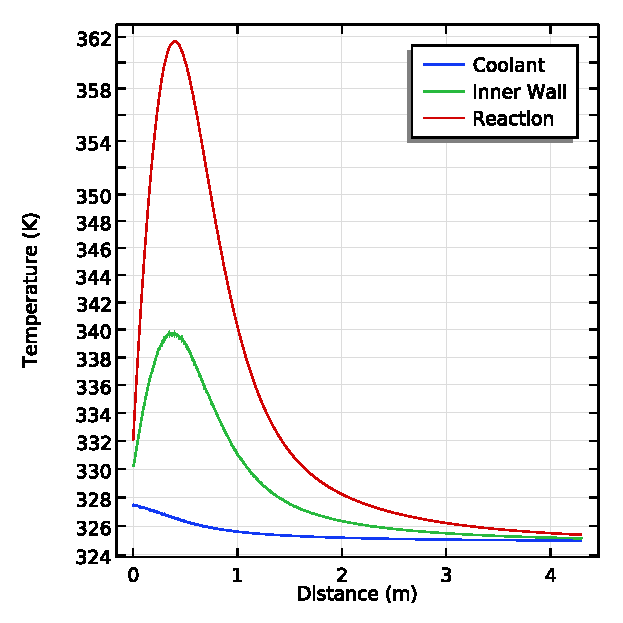
\includegraphics[width=\linewidth]{figures/temperature-lines-countercurrent.eps}
        \caption{Temperature profiles for counter-current secondary cooling water flow. Compare to \cref{fig:comsol-temperature:lines} (co-current flow).}
        \label{fig:comsol-temperature:lines:countercurrent}
    \end{minipage}\hfill
    \begin{minipage}[t]{0.45\linewidth}
        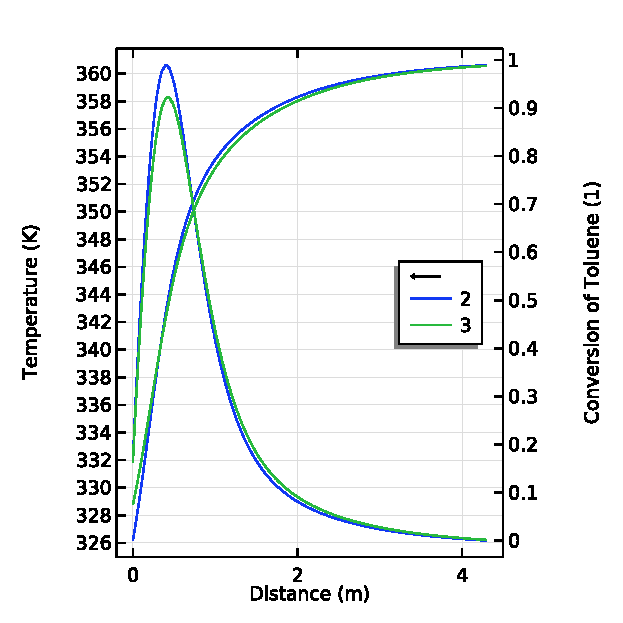
\includegraphics[width=\linewidth]{figures/S3-T-X.eps}
        \caption{Effect of changing nitric acid molar ratio on temperature and conversion profiles in reactor.}
        \label{fig:comsol-S3-T-X}
    \end{minipage}
\end{figure}

\subsubsection{\ch{HNO3} : Toluene inlet ratio}

\ch{HNO3} : Toluene molar ratio of 2 and 3 were investigated to achieve 98\% conversion in the shortest reactor length possible. Nitric acid is always kept in excess to maximise the formation of nitronium ion on the catalyst surface. Conversely, if the toluene is in excess, it will block the acid sites on the catalyst which obstructs the formation of nitronium ions \ref{vassena_selective_1999}.

The results in \cref{fig:comsol-S3-T-X} showed that increasing the \ch{HNO3} : Toluene molar ratio from 2 to 3 had a negligible effect on the conversion of toluene. This suggests that the surface of the catalyst had already been fully saturated. Therefore, increasing molar flowrate of nitric acid further would not enhance the conversion of the nitration reaction, but would instead lead to higher OPEX costs of supplying nitric acid to the reactor. It could also complicate the separation process of the 3 nitrotoluene isomers downstream. 

As safety is one of the key priorities of Nitroma in all decision making, the maximum temperature in the reactor were also analysed for both cases before making a final decision. Both cases were found to be below the safe temperature limit of \SI{363}{\K}, hence, a molar flowrate ratio of 2 was selected.

\subsubsection{Number of tubes}
A sensitivity analysis was performed on the number of reactor channels, shown in \cref{fig:S5-T-X}. An interesting point to note is that increasing number of tubes raises the average temperature as the peak temperature is more broad and spread out across the reactor channel. Although this would suggest that the rate of reaction and conversion would be higher, the opposite was observed. This can be explained by the decrease in volumetric flowrate per tube as the number of tubes increases. The effect of longer residence time in each channel outweighs the effect of higher average temperature in each channel. As a result, having more channels increases the overall conversion while reducing the peak temperature.

An optimal number of 7 tubes was chosen as it provides the lowest maximum temperature at 360K and spends a comparatively short length at a maximum temperature, which will reduce the occurrence of a thermal runaway. The targeted conversion of \SI{98}{\percent} can be achieved well within \SI{98}{\percent} of reactor length. 

The optimal number of tubes of 7 was also chosen based on the centered hexagonal number rule \cref{eqn: hexagon} which has practical usage in industry for maximising tube bundles into large cylindrical containers \cite{noauthor_realiable_2018}. 
\begin{equation}
    n^3 - (n-1)^3 = 3n(n-1)+1
    \label{eqn: hexagon}
\end{equation}
where $n$ represents the sequence of hexagonal number. The further explanation on the heat transfer benefits will be discussed in Section \ref{sec:reactortube}.

\begin{figure}[h]
    \begin{minipage}[t]{0.45\linewidth}
        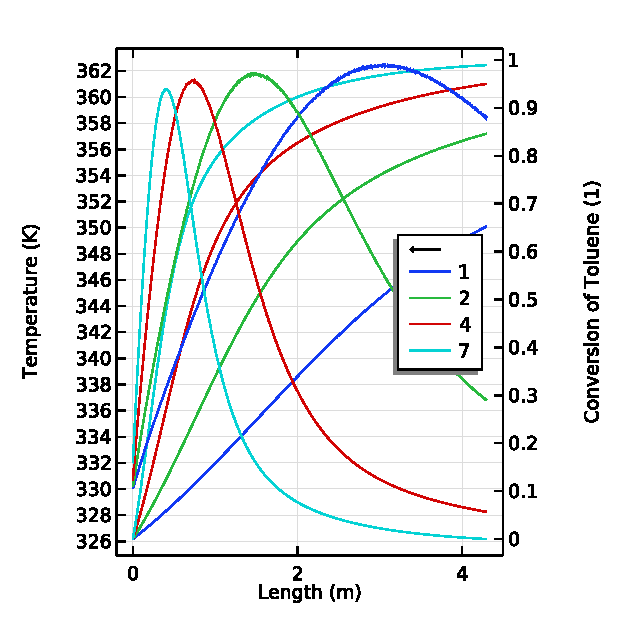
\includegraphics[width=\linewidth]{figures/S5-T-X.eps}
        \caption{Effects of changing number of tubes on reactor performance}
        \label{fig:S5-T-X}
    \end{minipage}\hfill
    \begin{minipage}[t]{0.45\linewidth}
        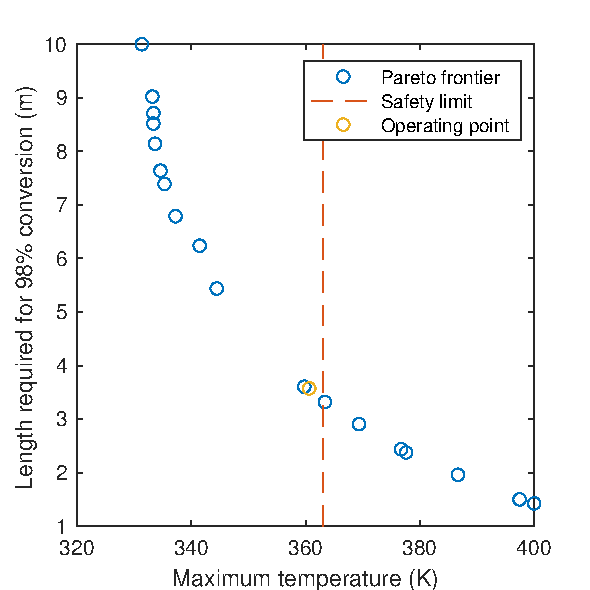
\includegraphics[width=\linewidth]{figures/comsol-pareto.pdf}
        \caption{Pareto frontier for reactor performance-safety tradeoff}
        \label{fig:comsol-pareto}
    \end{minipage}\hfill
\end{figure}

\subsubsection{Pareto frontier}
A Pareto frontier illustrating the tradeoff between reactor performance (i.e. minimising the length required to reach the target \SI{98}{\percent} conversion) and safety (i.e. minimising the maximum temperature reached within the reactor, related to the risk of thermal runaway) was derived using the MATLAB genetic algorithm function \texttt{gamultiobj} and is shown in \cref{fig:comsol-pareto}. The genetic algorithm varied the specification of the cooling system, namely the diameter and mass flow through the secondary cooling tube, and inlet temperature for both primary and secondary cooling. The operating point was selected to maximise reactor performance whilst still respecting the conservative \SI{90}{\celsius} thermal limit.

\subsubsection{Coolant temperature}
\label{sec:coolanttemp}
A sensitivity analysis was performed on the cooling water inlet temperature as temperature control was deemed the most important parameter for safety and performance evaluation. The length of reactor required was found to be quite sensitive to changes in inlet cooling temperature. Any changes in temperature would have a noticeable knock-on effect on the rate of reaction since the nitration process is sensitive to temperature \cite{chen_experimental_1998}. The region of interest in \cref{fig:comsol-S4-CW-X-T} is between \SI{325}{\K} \pm \SI{5}{\K}. Such a large fluctuation in temperature is unlikely to happen as the cooling water is sourced from a mixture of used cooling water streams across the plant and fresh cooling water. For each cooling stream to have a significant effect on the overall mixed cooling water stream temperature, there needs to be a significant deviation in the unit operations. The safety alarm systems in Nitroma's plant would alert the operators if that happens, therefore there is a low risk for the cooling water temperature to fluctuate by \pm \SI{5}{\K}. However, a conservative approach is taken when designing the HEX reactor. In the ideal scenario where the cooling water temperature does not fluctuate, a conversion of 98\% can be achieved in 3.6m as shown in \cref{fig:comsol-conversion}. When taking into account the maximum deviation of \pm \SI{5}{\K}, the reactor length is extended and the final reactor length is determined to be \SI{4.2}{\metre}. The summary of cooling water stream used in the HEX reactor can be found in \cref{tab:cwtable}.

\begin{figure}[h]
    \begin{minipage}[t]{0.45\linewidth}
        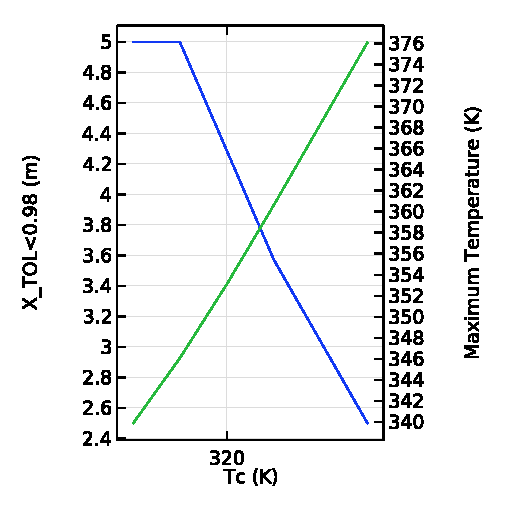
\includegraphics[width=\linewidth]{figures/S4-CW-X-T.eps}
        \caption{Effect of CW temperature on distance required to reach 98\% conversion (blue) and max T (green). Maximum reactor length is capped at 5m to prevent an excessively long reactor.}
        \label{fig:comsol-S4-CW-X-T}
    \end{minipage}\hfill
    \begin{minipage}[t]{0.45\linewidth}
        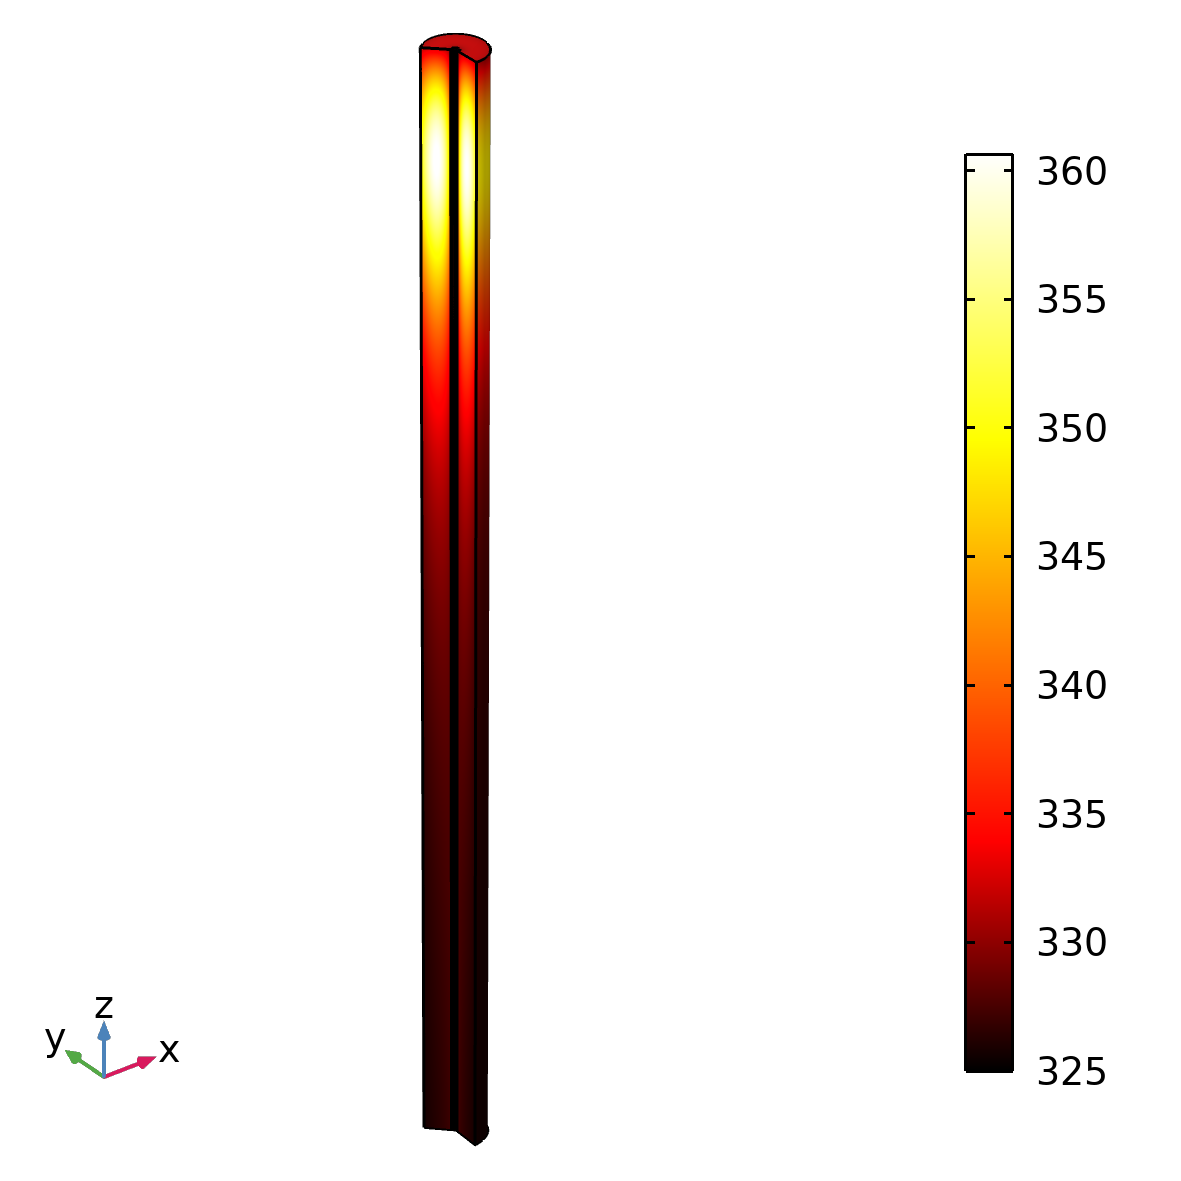
\includegraphics[width=\linewidth]{figures/temperature-surface.png}
        \caption{Temperature with external and internal cooling}
        \label{fig:comsol-temperature:surface}
    \end{minipage}
\end{figure}

\subsection{Final results}
\label{finalresults}
Using the optimised parameter values above, the reaction was simulated in the HEX nitration reactor. It showed robust performance by meeting the desired safety and reaction performance benchmark.

As illustrated in \cref{fig:comsol-conversion}, the reactor sees a sharp rise in conversion of \approx \SI{80}{\percent} in the first \SI{1}{\metre} of reactor before achieving the remaining \SI{20}{\percent} in the next \approx 3m. This can be explained by the rate of reaction as shown in \cref{fig:comsol-performance:r_TOL}. As high concentrations of reactants are first mixed together at the inlet of the reactor, the reaction proceeds at the highest rate in the first \SI{0.5}{\metre} before gradually decreasing after that. This results in a spike in temperature (\cref{fig:comsol-temperature}) since the reaction is an exothermic process, but the temperature does not continue on an upwards trajectory. This is due to the combined effect of having lower remaining concentration of reactants and efficient heat removal from cooling water which help keep the temperature below the safe temperature limit of \SI{363}{\K}. 

An interesting occurrence can be pointed out in \cref{fig:comsol-temperature:radial}. The figure shows the radial temperature profile at the slice of the reactor with the highest temperature. The temperature of the reaction fluid followed an asymmetrical parabola course due to the different heat flux across the inner and outer sides of the reaction annulus. A maximum temperature of \approx \SI{360.5}{\K} was located somewhere in the middle of the reaction annulus. Without either of the external or internal cooling water, the maximum temperature within the reactor would have increased well above \SI{363}{\K}, and hotspot would be found in the radial centre or the channel walls respectively . This emphasises the importance of Nitroma's novel triple concentric tube arrangement to achieving a safe and efficient reaction.

Overall, a \SI{98}{\%}conversion that is desired for the nitration reaction was achieved within the reactor. As expected, the more valuable ONT and PNT were produced in much greater amounts as compared to MNT. These products are later fed to other parts of Nitroma's plants to be converted to final products to be sold.

\begin{figure}[p]
    
    \begin{minipage}{\linewidth}
        \centering
        \begin{subfigure}{0.42\linewidth}
            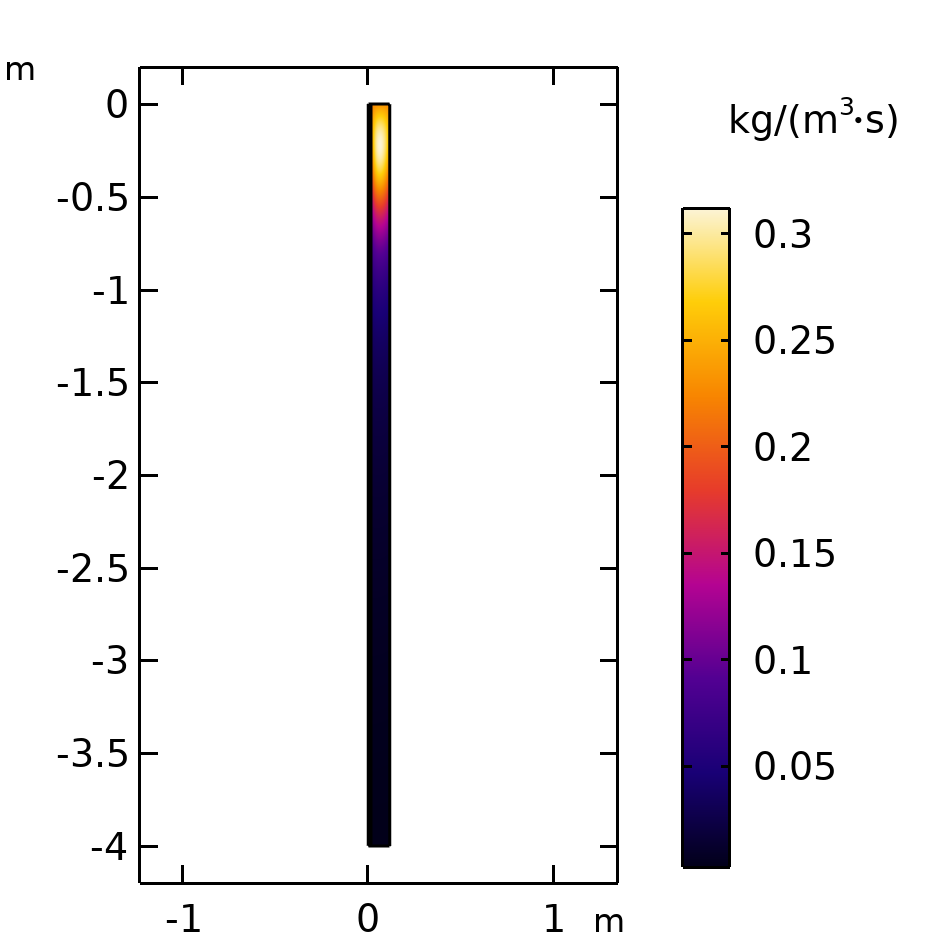
\includegraphics[width=\linewidth, scale=0.5]{figures/r_TOL.png}
            \caption{Rate of Toluene reaction}
            \label{fig:comsol-performance:r_TOL}
        \end{subfigure}\hspace{\floatsep}
        \begin{subfigure}{0.42\linewidth}
            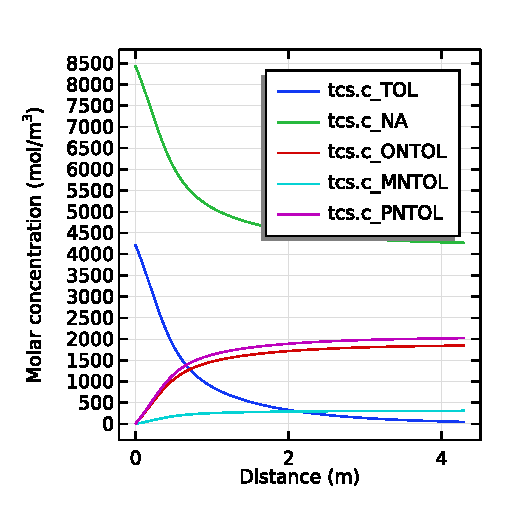
\includegraphics[width=\linewidth, scale=0.5]{figures/concentration.eps}
            \caption{Concentration profile within reactor}
            \label{fig:comsol-performance:concentration}
        \end{subfigure}
        \caption{Reactor performance}
        \label{fig:comsol-performance}
    \end{minipage}
    \vspace{\floatsep}
    
    \begin{minipage}{\linewidth}
        \centering
        \begin{subfigure}{0.42\linewidth}
            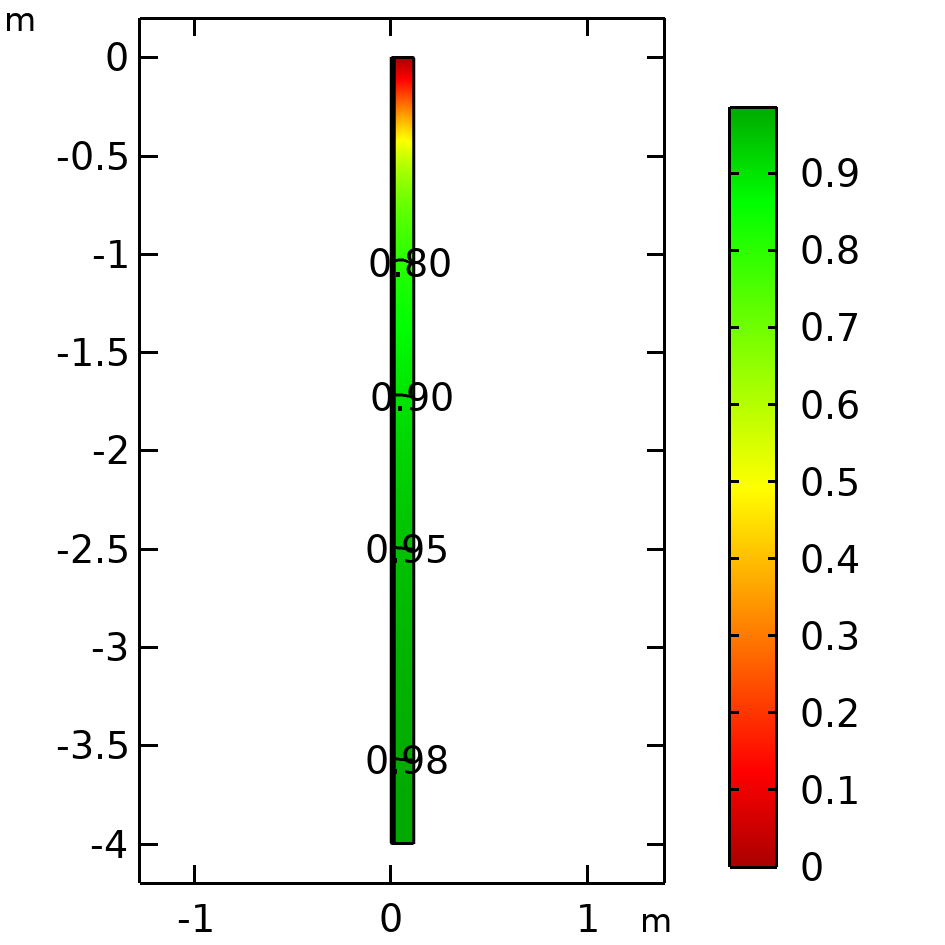
\includegraphics[width=\linewidth, scale=0.3]{figures/conversion-surface.png}
            \label{fig:comsol-conversion:surface}
        \end{subfigure}\hspace{\floatsep}
        \begin{subfigure}{0.42\linewidth}
            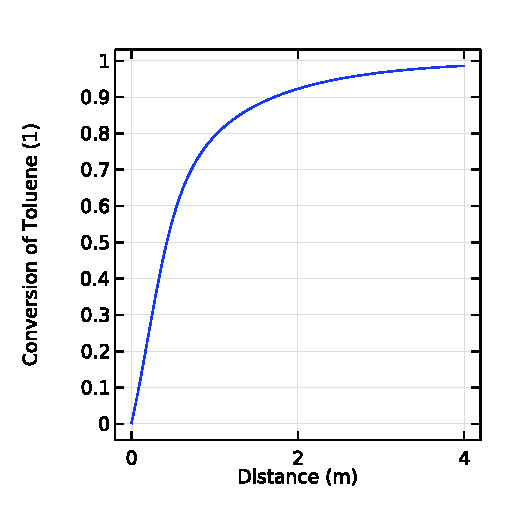
\includegraphics[width=\linewidth, scale=0.3]{figures/conversion-line.eps}
            \label{fig:comsol-conversion:line}
        \end{subfigure}
        \caption{Conversion of toluene across reactor length}
        \label{fig:comsol-conversion}
    \end{minipage}
    \vspace{\floatsep}
    
    \begin{minipage}{\linewidth}
        \centering
        \begin{subfigure}{0.42\linewidth}
            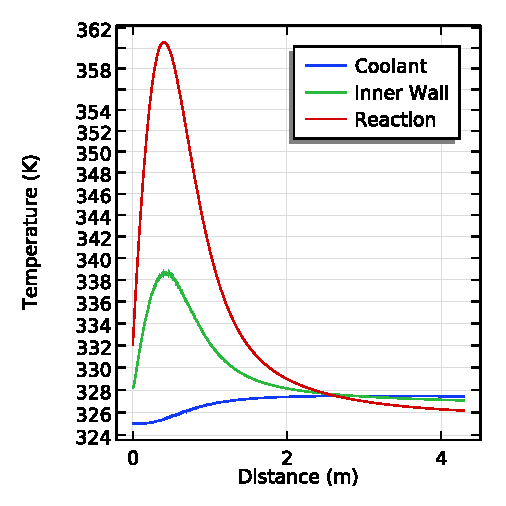
\includegraphics[width=\linewidth]{figures/temperature-lines.eps}
            \caption{$T(z)$ within each section}
            \label{fig:comsol-temperature:lines}
        \end{subfigure}\hspace{\floatsep}
        \begin{subfigure}{0.42\linewidth}
            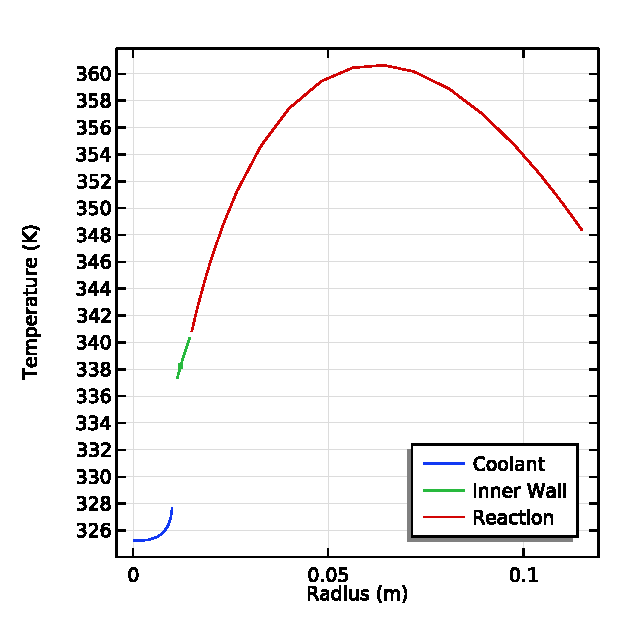
\includegraphics[width=\linewidth]{figures/Tr-maxT.eps}
            \caption{$T(r)$ at $T = \max(T)$}
            \label{fig:comsol-temperature:radial}
        \end{subfigure}
        \caption{Temperature profiles in reactor}
        \label{fig:comsol-temperature}
    \end{minipage}
    
\end{figure}
